\chapter{Introduction}\label{CH:introduction}

\cck{test CCK comment in favorite pen color}

\jdp{How does the sun affect us and why do we care?}
The Sun is arguably the most relevant astrophysical object to humanity.
Its distance from the earth defines a Goldilocks zone (not too hot, not too cold) in which human life can exist.
Most of the energy that we use daily can be attributed to the sun, from the obvious solar power, to wind and hydro power (driven by weather created by the sun), to fossil fuels formed from the decay of organic organisms of the past.
The rising and setting of the sun defines the daily human experience.
Despite our reliance on the sun it is often underappreciated by us and overlooked by physicists who choose to study supposedly more `sexy' astrophysical objects much further away.

In addition to being essential to life on earth, the sun is very violent and energetic.
The sun is constantly blasting the earth with radiation and high energy particles.
Luckily the earth's atmosphere and magnetic field protects us from both.
The earth's atmosphere absorbs a large portion of the solar radiation, some of which (x-ray and ultraviolet) can be quite harmful to humans.
The earth's magnetic field steers most energetic particles around earth.
Despite these protections we are not immune to the sun's effects.
Satellites are vulnerable to the shower of energetic particles from the sun, which can damage computer chips and lead to charge build up that affects the electronics within.
Periods of intense solar activity can heavily perturb the earth's magnetic field, causing geomagnetic storms.
These geomagnetic storms can cause variations in the Ionosphere, a charged layer of our atmosphere, that can negatively effect radio communication and GPS.
Astronauts beyond the protection of the earths magnetic field exposed to solar energetic particles produced during solar flares would receive large doses of radiation, equivalent to hundreds of dental x-rays, that can lead to radiation poisoning \citep[][and references therein]{Temmer2021}.
As our technology advances, and our society becomes less confined to the surface of the earth, it is becoming increasingly important that we improve our understanding of, and our ability to predict, the activity of our closest star.


 

 \jdp{Where does the Sun's energy and magnetic field come from?}
 
\begin{figure}
	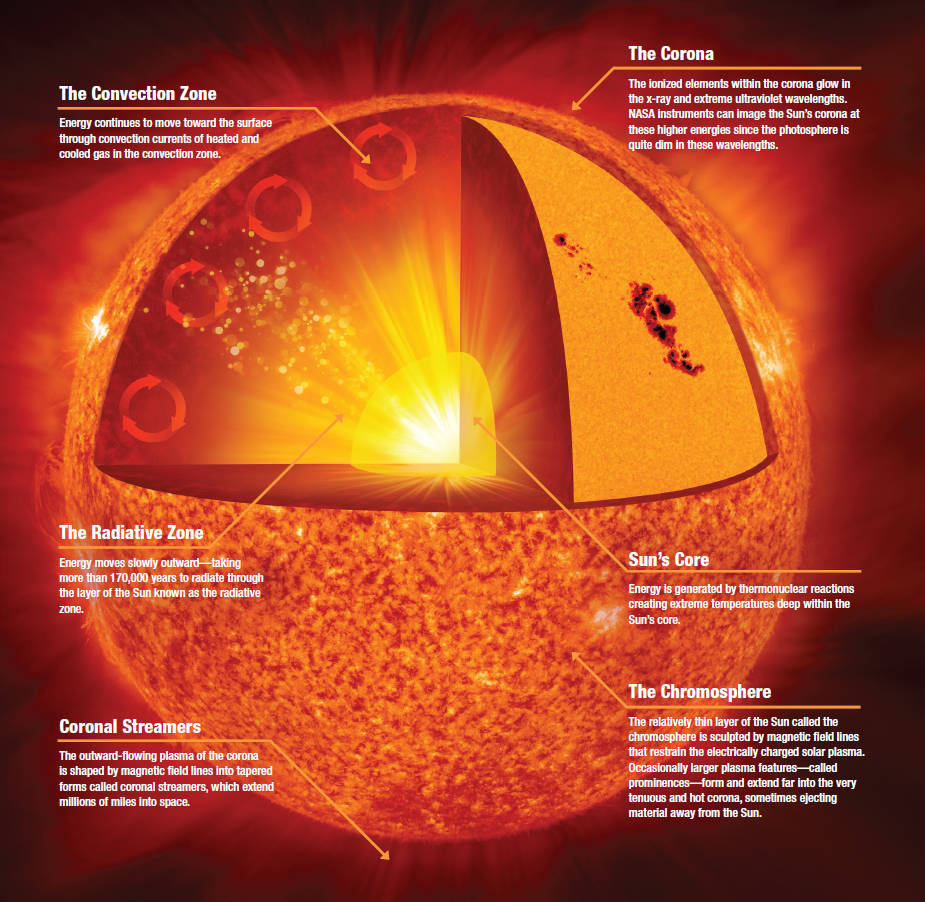
\includegraphics[width=\textwidth]{solar-anatomy.jpg}
	\caption{Considering borrowing this from NASA. Not yet integrated into the text.}
\end{figure} 
 
Energy produced in the sun originates from nuclear fusion in the core, where temperatures reach approximately 15 million Kelvin.
From there energy moves outward through the solar interior until reaching the solar surface which has an average temperature of approximately 6600 Kelvin  \citep{SolarPhysicsOverview}. 
The solar interior consists of three layers: the core, the radiation zone, and the convection zone.
The \emph{radiation} and \emph{convection} zones are each named after their dominant mode of energy transfer.
The transition between the two zones, referred to as the tachocline, is where temperature gradient becomes steep enough that the solar plasma becomes unstable to convection, and is likely where the solar magnetic field originates \citep{SolarPhysicsOverview}.
At the solar surface, and within the convection zone, the sun undergoes differential rotation, with plasma rotating more quickly near the equator than the poles.
It is the combination of convective motions, and differential rotation, that are understood to structure the suns global magnetic field \citep{Parker1979,Priest2014,JudgeBook}.
Magnetic field lines produced in the convection zone rise through the solar surface, up into the solar atmosphere, where they become the dominant player and contribute to a host of spectacular solar events, including those studied in this thesis.

%, from which almost all the energy produced in the core radiates away\citep{JudgeBook}.

\jdp{The Solar Atmosphere}
The solar surface, referred to as the photosphere, is the base of the solar atmosphere and is defined as the point where photons can escape into space without being reabsorbed by surrounding plasma \citep{Priest2014}.
It is important to note that the photosphere isn't really a surface, but a thin region of plasma with steadily decreasing density and temperature.
Despite this the height of the photosphere is very thin in comparison to the solar radius, $\approx 300$\, km compared to the $\approx$ 700,000\, km solar radius, and therefore looks very crisp when observed from earth \citep{JudgeBook}.
It is at the edge of the photosphere where the sun reaches an average temperature minimum of $\approx4400$ Kelvin \citep{SolarPhysicsOverview}.
The rest of the solar atmosphere consists of (in order of increasing radius) the chromosphere, transition region, and corona.
The chromosphere, named for the red light it produces that is visible with the naked eye during total solar eclipses, extends approximately 1500 km in height \citep{SolarPhysicsOverview}.
Within the chromosphere the average temperature rises from the temperature minimum to approximately 10,000  Kelvin.
At the edge of the Chromosphere the average temperature increases rapidly to average temperature of approximately 1 million Kelvin in the outer most layer of the atmosphere, called the corona \citep{SolarPhysicsOverview}.
The thin region, less than 100 km thick \citep{Priest2014}, where this transition occurs is appropriately named the transition region.

While it is easiest to think of the solar atmosphere as occurring in one dimensional static layers, in reality it is very structured and dynamic.
Above the photosphere, the magnetic field generated in the convection zone expands into a vast canopy of closed loops, with their ends anchored down in the photosphere, as well as open field lines extending out into space.
Hotter plasma traces these field lines, allowing us to visualize the complex magnetic field.
These magnetic structures have been assigned a whole zoo's worth of names by solar physicists, and are subject to continuous study and debate.
Regardless, there presence and evolution in images of the solar atmosphere indicate the dynamic and three dimensional nature of the solar atmosphere, making it a very rich area of study.


 
\jdp{What are we looking for when we study the solar atmosphere and why?}
The solar atmosphere is interesting and worth studying for two main reasons, it is hot and it is violent.
As is described above, the solar atmosphere is hotter than the solar surface!
Since the roughly 6000 degree photosphere is incapable of heating the corona to a million degrees, the energy has to come from somewhere else.
A likely source of this energy is the sun's magnetic field \citep{Priest2014}.
Beyond the surface of the sun the solar plasma transitions from being fluid dominated, to magnetically dominated.
Whether a plasma is fluid or magnetically dominated depends on the ratio of its fluid pressure, $p$, to its magnetic pressure, $p_\text{mag}$, or plasma beta, where,
\begin{equation}
	\beta = \frac{p}{p_\text{mag}} = \frac{nk_\text{B}T}{B^2 / 2\mu_0},
\end{equation}
and $n$ is the plasma density, $T$ its temperature, and $B$ the magnetic field strength.
A plasma with $\beta>1$ can be manipulated by fluid motion, as is the case in the photosphere and below.
As plasma density decreases in the chromosphere and beyond, areas with strong magnetic field strength have $\beta<1$.  
In this portion of the atmosphere the magnetic field dominates, and the charged solar plasma is ``frozen in'' to the magnetic field.
Therefore magnetic field motions begin to dictate plasma motion \citep{Priest2014}.

In the solar atmosphere, the magnetic field is complicated and continuously evolving.
Fluid motions in the photosphere, driven by the convection and differential rotation, shuffle the base of magnetic loops and open filed lines, known as foot points, changing the field above.
Also, new magnetic field lines are constantly being brought to the surface, a process called flux emergence, that interact with the field above.
As the magnetic field is shuffled around, and interacts with emerging flux, it is twisted and tangled gaining energy, until, somewhat suddenly instability sets in.
%This interplay between a fluid dominated photosphere and a magnetically dominated corona leads to a host interesting solar events.
%The photosphere constantly evolves like a pot of boiling water, as hot plasma is convected to the surface and cooler back down.
%This motion causes the base of magnetic field lines anchored in the photosphere, referred to as foot points, to be pushed around.
%Meanwhile, the magnetic field in the corona that has found equilibrium is happy and would prefer to stay the way they are.
%Foot point motion at the photosphere slowly begins to twist and tangle the magnetic field above, imparting more and more energy into it, until suddenly instability sets in.
These instabilities allow the magnetic field lines to reconfigure themselves into a lower energy state, a process referred to as magnetic reconnection \citep{Parker1957,Petschek1964}.
When field lines reconnect, energy stored in the magnetic field is quickly converted to kinetic energy, capable of accelerating plasma to velocities much greater that would be possible through thermal means.
The speed limit for a fluid dominated plasma is the speed of sound.
Motion generated by the magnetic field obeys a different speed limit, the Alfv\' en velocity, which is the speed at which a wave travels along a magnetic field line.
In areas of strong magnetic field the Alfv\' en velocity can be an order of magnitude faster than the local sound speed in the plasma \citep{Priest2014}.
Observations of velocities much greater than the sound speed during solar eruptions indicate the important roll of the magnetic field and magnetic reconnection.
Also, the correlation between areas of strong magnetic field and eruptive activity, with the hotter parts of the corona, make the solar magnetic field a strong candidate for the excess temperature of the solar atmosphere.


\jdp{How do we study the solar atmosphere?}
Almost everything we know about the sun comes from examining the light it produces.
Advances in our understanding of atomic physics and quantum mechanics have allowed us to collect light from the sun, using a variety of techniques, and from it determine things like plasma temperature, density, velocity, and elemental content, as well as the magnetic field strength.
All of this information can then be pieced together to form a more complete picture of solar events so that we can better inform and test our models and understanding.

The solar atmosphere, being a plasma, consists of charged particles including free electrons and ions.
As electrons and ions interact and collide, they experience changes in energy. 
In order to conserve energy, excess energy needs to be either stored, by exciting bound electrons to higher energy states, or released in the form of radiation.
Energy is radiated away as a photon, a discrete packet of light, with a specific wavelength, $\lambda$, where the energy,
\begin{equation}
	E = \frac{hc}{\lambda},
\end{equation}
$h$ is Plank's constant, and $c$ is the speed of light.
Therefore, by measuring the wavelength of a photon, we know its energy.
Energy stored in an ion's bound electron is also eventually emitted as a photon when the bound electron transitions from an excited state, to a more stable one.
Quantum mechanics tells us that these transitions occur in discrete steps.
Therefore, the wavelength of a measured photon can also tell us what kind of ion produced it.
Since ions in the solar plasma are often moving, either because of thermal motions or changes in the magnetic field, the wavelength of emitted photons are often Doppler shifted.  
Just as train whistle sounds higher or lower pitched depending on if the train is moving toward or away from you, emitted photons have shorter or longer wavelengths depending on the ions velocity.
Slight deviations from a photons expected wavelength tell us the ion's velocity,
\begin{equation}
	v = c \frac{\lambda - \lambda_0}{\lambda_0},
\end{equation}
where $\lambda$ is the measured wavelength and $\lambda_0$ is the emitted wavelength at zero velocity.
Photons of shorter wavelength are referred to as blue shifted, an analogy to visible light, and longer wavelengths red shifted.
In solar physics the convention is to define the positive direction as away from us and toward the sun, therefore blue shifted photons have negative velocity and are traveling toward us, and red the opposite.

Light emitted from the sun comes in a wide ($\approx3000$\, nm) range of wavelengths, referred to as the solar spectrum, with it's peak emission being visible light ($\approx400-700$\, nm). 
The solar spectrum is broadly peaked around visible light, but zooming in reveals many smaller peaks and dips at various wavelengths. \jdp{I might need a figure for this.}
These peaks and dips are from ions emitting or absorbing photons at specific wavelengths, referred to as spectral lines, are the key to isolating and studying different portions of the solar atmosphere.
Using filters we can isolate narrow wavelength ranges and image the sun only in that range.
Images of the photosphere can be captured from earth, since visible light easily passes through the Earth's atmosphere.
As temperature increases from the photosphere up through the rest of the solar atmosphere, the sun emits generally shorter wavelengths. \jdp{True in general?}
These shorter wavelengths, from ultraviolet to x-ray, are readily absorbed by the Earth's atmosphere, and therefore must be imaged from space. 
The currently operating Atmospheric Imaging Assembly \citep[AIA:][]{} on board the Solar Dynamics Observatory (a satellite with multiple solar instruments), uses narrow filters to image the sun in several different Extreme Ultraviolet (EUV) wavelength ranges aimed at isolating bright spectral lines emitted produced in the solar atmosphere.
Figure \ref{fig:AIA} shows 4 of these images centered around \jdp{x} wavelengths.
From quantum mechanics we know these wavelengths come from \jdp{x} ions that occur most often at \jdp{temperatures}.
This allows us to image the solar atmosphere at various heights and temperatures so we can better understand the structure of solar features and events.
Unfortunately most filters aren't narrow enough to truly isolate individual spectral lines or portions of them.
Therefore in order to increase our spectral resolution we use a different instrument, the spectrograph.

The spectrograph is a fundamental tool for better understanding light coming from the sun. 
Spectrographs use diffraction gratings to disperse based on it's wavelength, allowing you to examine the spectral content.
Typically light traveling through a spectrograph will be focused through a slit, a very narrow strip for light to travel through, prior to being dispersed by a diffraction grating.
These are referred to as slit spectrographs.  
When used to image the sun, this results in an image of practically pure spectral signal over taken from a very narrow strip of sun in the direction perpendicular to the slit.
The Interface Region Imaging Spectrograph \citep[IRIS:][]{} is currently operating satellite based slit spectrograph imaging the sun.
Slit spectrographs like IRIS build spectrally resolved images, an image of the sun with spectral information at every pixel, by scanning the slit over a wider field of view, referred to as rastering.
Images from a rastered slit spectrograph can achieve very high spatial and spectral resolution over a decent size field of few.
For example, a 320 step raster from IRIS has a \jdp{???} spatial and spectral resolution over a \jdp{???} field of view.
The down side of rastering a slit spectrograph is that a full exposure is required at every position, each of which take several seconds at minimum if not tens of seconds.
This results in an image that was taken over the course of minutes to hours.
For more static solar scenes with less activity, this trade off can have little affect.
Unfortunately, many solar eruptions evolve on second timescales, causing your scene to constantly change as you try to capture an image of it, often resulting in the slit being pointed away from an event of interest.

An alternate approach is to remove the slit, and disperse an image over a much larger field of view using a diffraction grating, often referred to as a slitless spectrograph.
Images from a slitless spectrograph have overlapping spatial and spectral information in every pixel.
Therefore, in order to capture a spectrally resolved image of the sun, images from multiple slitless spectrograph channels need to be combined.
These instruments, referred to as Computed Tomography Imaging Spectrographs (CTIS), use the same principle as a CT (Computed Tomography) scan in a doctors office that combine a series of unique two dimensional images taken from different angles, to form something three dimensional.
The primary difference between a CTIS instrument and a CT scan is that the goal of a CT scan is the capture a data cube with three spatial dimensions, $I(x,y,z)$, whereas a CTIS instrument returns a cube with two spatial dimensions and one spectral dimensions, $I(x,y,\lambda)$.

Compared to slit spectrographs CTIS instruments compromise spatial and spectral resolution for increased field of view and a faster temporal cadence.
Since multiple channels can image a scene simultaneously, spectrally resolved images can be formed at every exposure, taking seconds instead of minutes or hours.
Although, since we can only fit a limited number of channels, and there is an overlap in spatial and spectral information at every pixel, CTIS instruments have lower spatial and spectral resolution.
The Multi-Order Solar Extreme Ultraviolet Spectrograph \citep[MOSES:{}][]{Fox2010} and Extreme ultraviolet Snapshot Imaging Spectrograph\citep[ESIS:][]{}, are two CTIS instruments developed at MSU have have a resolution of \jdp{??} and \jdp{???} respectively. \jdp{rethink if this is even needed.}

\jdp{Thesis Outline}
The content of this thesis is divided into three different chapters.  
The first chapter explores data from the first flight of the ESIS sounding rocket launch, the second describes a method by which to quantify the total spectral content in images from the first light of MOSES in February of 2006, and the third develops a model of magnetic reconnection used to describe the observation of elliptical motion in a flare ribbon observed by \citet{Brannon2015}.

A team from Montana State successfully launched the ESIS sounding rocket from White Sands Missile Range on September 30th, 2019.
We describe the history of CTIS instruments observing the sun, and there advantages 






	




